\documentclass{article}
\usepackage[utf8]{luainputenc}
\usepackage[T1]{fontenc}
%\usepackage[a4paper,margin=0.75in, bottom=1in]{geometry}
\usepackage{fullpage}
\usepackage{listings}
\usepackage{courier}
\usepackage{amsmath}
\usepackage{amssymb}
\usepackage{enumerate}
\usepackage{graphicx}
\usepackage{hyperref}

\begin{document}
	
	\setlength{\parindent}{0em} 
	
	\hrulefill
	\begin{center}
		\bfseries % Fettdruck einschalten
		\sffamily % Serifenlose Schrift
		\begin{huge}
			GTI: Grundlagen der Theoretischen Informatik
		\end{huge}\\
		\begin{Large}
			Sommersemester 2017, 6. Übungsblatt
		\end{Large}\\
		\begin{small}
			Valentin Wolf, Luis Herrmann; Tutor: Kristin Knorr; Mo 12:00-14:00
		\end{small}
		
		\vspace{-10pt}
	\end{center}
	\hrulefill
	
\section*{Aufgabe 1 - \textit{Nochmal Pumping Lemma}}

Wie betrachten die Sprache $L := \{c^k a^l b^l | k,l \ge 0 \} \cup \{a,b\}^*$ über das Alphabet $\Sigma = \{a,b,c\}$. Wir zeigen, dass $L$ die Bedingung aus dem Pumping-Lemma für reguläre Sprachen erfüllt. Zur Erinnerung: Sei $L$ eine reguläre Sprache. Dann besagt das Pumping-Lemma $\exists n\ge 1 \forall z\in L , |z| \ge n \exists $ Zerlegung $z = uvw$ mit $|uv| \le n, |v| \ge 1 \forall i \in \mathbb{N}_0: uv^iw \in L$.

Wir wählen $n =1 $. Dann gilt offenbar für beliebige $z \in L $: $z = c^k a^l b^l$ mit $|z| = k+2l$ oder $z = \{a,b\}^{|z|}$. Betrachten wir zunächst den 1. Fall. Offenbar gibt es für $n=1$ nur eine gültige Zerlegung von $z$, nämlich $uv = c$ (impliziert $v = c$) und $w = c^{k-1}a^l b^l$. Nun gilt aber:
\begin{equation}
	uv^i w = c^i c^{k-1} = c^i c^{k-1}a^l b^l = c^{k+i-1}a^l b^l \in L \forall i\in \mathbb{N}_0 \forall k\ge 1
\end{equation}

Für $z = \{a,b\}^{|z|}$ ist das Pumping-Lemma trivialerweise erfüllt, denn $\{a,b\}^*$ ist eine reguläre Sprache, also ist das Pumping-Lemma für alle Wörter aus der Sprache erfüllt, wobei diese gerade die Form $\{a,b\}^{|z|}$ haben. Also ist das Pumping-Lemma für alle Wörter aus der Sprache $L$ erfüllt.\\

L ist aber keine reguläre Sprache. Das überlegt man sich am besten über die Myrill-Nerode-Relation: Betrachte Wörter $w_l := c^k a^l$ und $w_m := c^k a^m$, sodass $w_l,w_m \not\in L$. Wählen wir nun das Suffix $z = b^l$, so gilt $w_lz = c^k a^l b^l \in L$, aber $w_mz = c^k a^l b^m \not\in L$. Das heißt, zwei Worte $w_l, w_m$ sind für bel. $l \ge 0, l \neq m$ nicht äquivalent bezüglich der Nerode-Relation und somit muss es unendlich viele Äquivalenzklassen geben. Damit ist die Sprache $L$ gemäß Satz von Myrill-Nerode nicht regulär.

\section*{Aufgabe 2 - \textit{Abschlusseigenschaften}}

Seien $L, L_1, L_2$ entscheidbare Sprachen über $\Sigma$. D.h. die zugehörigen Charakteristischen Funktionen $\chi_L, \chi_{L_1}$ und $\chi_{L_2}$ sind Turing-berechenbar. Zur Erinnerung:
\begin{equation}
	\chi_L(w) := \begin{cases}
	1, &w \in L\\
	0, &\text{sonst}
	\end{cases}
\end{equation}

\begin{enumerate}
	\item Offenbar ist dann auch $L^C$ eine entscheidbare Sprache, denn die Boole'sche Negationsfunktion $\neg$ ist Turing-berechenbar. Indem man für ein beliebiges Wort $w \in \Sigma^*$ zunächst die Berechnung von $\chi_L(w)$ gemäß Programm der entsprechenden TM $M$ ausführt und anschließend die Ausgabe auf dem Band negiert hat man eine Turing-Maschine beschrieben, die $\chi_L^C$ berechnet, denn:
	\begin{equation}
		\forall w \in \Sigma^*: \chi_L^C(w) = \neg \chi_L(w) = \begin{cases}
		0, &w \in L \Leftrightarrow w \in L^C\\
		1, &w \not\in L \Leftrightarrow w \in L \text{ sonst}
		\end{cases}
	\end{equation}
	
	\item Ähnlich überlegt man sich, dass auch $L_1 \cup L_2$ entscheidbar ist, denn $\chi_{L_1}$ und $\chi_{L_2}$ sind nach Voraussetzung Turing-berechenbar, d.h. es gibt zugehörige TM $M_1$ und $M_2$, die die Funktionen berechnen. Dann lässt sich eine 2-Band-TM beschreiben, die als Eingabe ein Wort $w\in \Sigma$ auf Band 1 erhält, dieses auf Band 2 kopiert, und anschließend parallel die Berechnung $\chi_{L_1}(w)$ auf Band 1 gemäß Programm von $M_1$ und $\chi_{L_2}(w)$ auf Band 2 gemäß Programm von $M_2$ durchführt. Mit den Rückgabewerten wird dann $\chi_{L_1}(w) \lor \chi_{L_2}(w)$ berechnet und beispielsweise auf Band 1 geschrieben und es gilt gerade:
	\begin{equation}
		\forall w \in \Sigma^* : \chi_{L_1 \cup L_2}(w) = \chi_{L_1}(w) \lor \chi_{L_2}(w) = \begin{cases}
		1, &w\in L_1 \lor w\in L_2 \Leftrightarrow w \in L_1\cup L_2 \\
		0, &w \not\in L_1\cup L_2
		\end{cases}
	\end{equation}
	
	Da die zweistellige Boole'sche Funktion $\lor$ offensichtlich Turing-berechenbar ist, haben wir also eine Turing-Maschine charakterisiert, die $\chi_{L_1 \cup L_2}$ berechnet und die Sprache $L_1 \cup L_2$ ist somit entscheidbar.
	
	\item Um zu zeigen, dass $L_1\cap L_2$ entscheidbar ist, wendet man genau die gleichen Überlegungen wie für $L_1\cup L_2$ an, aber berechnet stattdessen $\chi_{L_2} \land \chi_{L_2}(w)$, wobei die zweistellige Boole'sche Funktion $\land$ offensichtlich Turing-berechenbar ist, und es gilt gerade:
	\begin{equation}
		\forall w \in \Sigma^* : \chi_{L_1 \cap L_2}(w) = \chi_{L_1}(w) \land \chi_{L_2}(w) = \begin{cases}
		1, &w\in L_1 \land w\in L_2 \Leftrightarrow w \in L_1\cap L_2 \\
		0, &w \not\in L_1\cap L_2
		\end{cases}
	\end{equation}
	
	Damit haben wir eine TM charakterisiert, die $L_1 \cap L_2$ entscheidet und die Sprache ist entscheidbar.
	
	\item Zuletzt zeigen wir, dass dann auch $L^*$ entscheidbar ist. Dazu nehmen wir an, wir kopieren das Eingabewort $w$ auf dem Band und führen auf der Kopie die Berechnung $\chi_L(w)$ durch. Falls die Berechnung 1 zurückgibt, sind wir fertig, denn $w \in L \Rightarrow w\in L^*$. Sonst ist folgender Fall zu betrachten:
	
	Angenommen $w\not\in L$, aber $w \in L^*$. Dann ex. $i \ge 1: w_1 .... w_i \in L \land w_{i+1}... w_n \in L^*$, denn sonst wäre $ \forall i\ge 1 : w_{1...i} \circ w_{i+1...n} \not\in L^*$.
	
	Die Idee zur Überprüfung von $w \in L^*$ durch eine TM ist also Folgende:
	\begin{enumerate}
		\item Prüfe $\forall i\ge 1$, ob $w_{1...i} \in L$.
		\item Falls nicht, verwerfe $w$, denn $w \not \in L$.
		\item Falls doch, prüfe ob $w_{i...n} \in L^*$.
	\end{enumerate}
	
	Die Rekursion über kleiner werdende Suffixe von $w$ wird wiederholt, bis ein Suffix verworfen wird, sodass $w\not\in L$ (und es wird 0 auf das Band geschrieben) oder bis für ein $1 \le j \le n$ gilt, dass $w_{j ... n} \in L$. Im letzten Fall wird $w$ akzeptiert, 1 auf das Band geschrieben und wir sind fertig.
	
	Auf die konkrete Umsetzung als TM gehen wir nicht ein, aber per Konstruktion ist klar, dass die Berechnung durch eine rekursive Funktion möglich ist und dass gemäß Church'scher These die entsprechende Funktion demnach auch Turing-berechenbar sein sollte.
	
\end{enumerate}

\section*{Aufgabe 3 - \textit{Schleifen}}

Eine Momentaufnahme in der Berechnung einer 1-Band-TM $(Q,\Sigma,\Gamma,q_0,\delta,\text{\textvisiblespace},F)$ ist definiert durch den Zustand des Bandes, der Kopfposition und durch den aktuellen Berechnungszustand $q \in Q$, den die Kontrolle einnimmt. Wenn die TM höchstens Bandzellen $1,...,s(n)$ besucht, dann gibt es für eine Bandalphabet $\Gamma$ also höchstens $|\Gamma|^{s(n)}$ Konfigurationen des Bandes, die möglich sind. Entsprechend sind höchstens $s(n)$ Kopfpositionen möglich. Bezüglich der Berechnungszustände kann sich die TM in höchstens $|Q|$ Konfigurationen befinden. Insgesamt ergeben sich somit höchstens
\begin{equation}
	|\Gamma|^{s(n)} s(n) |Q|
\end{equation}

mögliche Konfigurationen der TM. Diese muss also spätestens nach $|\Gamma|^{s(n)} s(n) |Q|$ Schritten in eine Schleife geraten.

\section*{Aufgabe 4 - \textit{Kodierte dfas}}

Wir zeigen, dass $L_\text{finite} := \{\langle A \rangle | A \text{ ist dfa und } L(A) \text{ ist endlich} \}$ ist eine entscheidbare Sprache. Dabei soll $\langle A \rangle$ eine geeignete Kodierung der Sprache sein.\\

\begin{itemize}
	\item Wie wir in der Vorlesung gezeigt haben gilt $A$ ist dfa gdw. $L(A)$ ist reguläre Sprache mit $L(A) := \{w \in \Sigma^* | \delta^*(w) \in F\}$. Also ist jede Kodierung eines dfa $A$ äquivalent mit der Kodierung einer regulären Sprache $L(A)$.
	
	\item Gemäß Definition lässt sich jede reguläre Sprache durch einen regulären Ausdruck darstellen. Also gibt es zu jedem dfa einen kodierenden regulären Ausdruck und $\langle . \rangle_\text{reg}$ ist eine geeignete Kodierung von dfas.
\end{itemize}

Offenbar ist $L(A)$ endlich gdw. der zugehörige reguläre Ausdruck $\alpha(L(A))$ keinen Kleene-Stern enthält. Wenn die dfas von $L_\text{finite}$ über einem Alphabet $\Sigma$ definiert sein sollen, können wir also die TM $M$, die $L_\text{finite}$ entscheidet, derart konstruieren, dass $\tilde{\Sigma} := \Sigma_\epsilon \cup \{\cup,{}^*, (,) \}$. Die Turing-Maschine braucht dann lediglich zu überprüfen, ob das übergebene reguläre Wort eine gültiger regulärer Ausdruck ist und dass es keinen Kleene-Stern enthält.

Eine Turing-Maschine, die dies leistet, wäre zum Beispiel folgende:

\begin{minipage}{\textwidth}
	\centering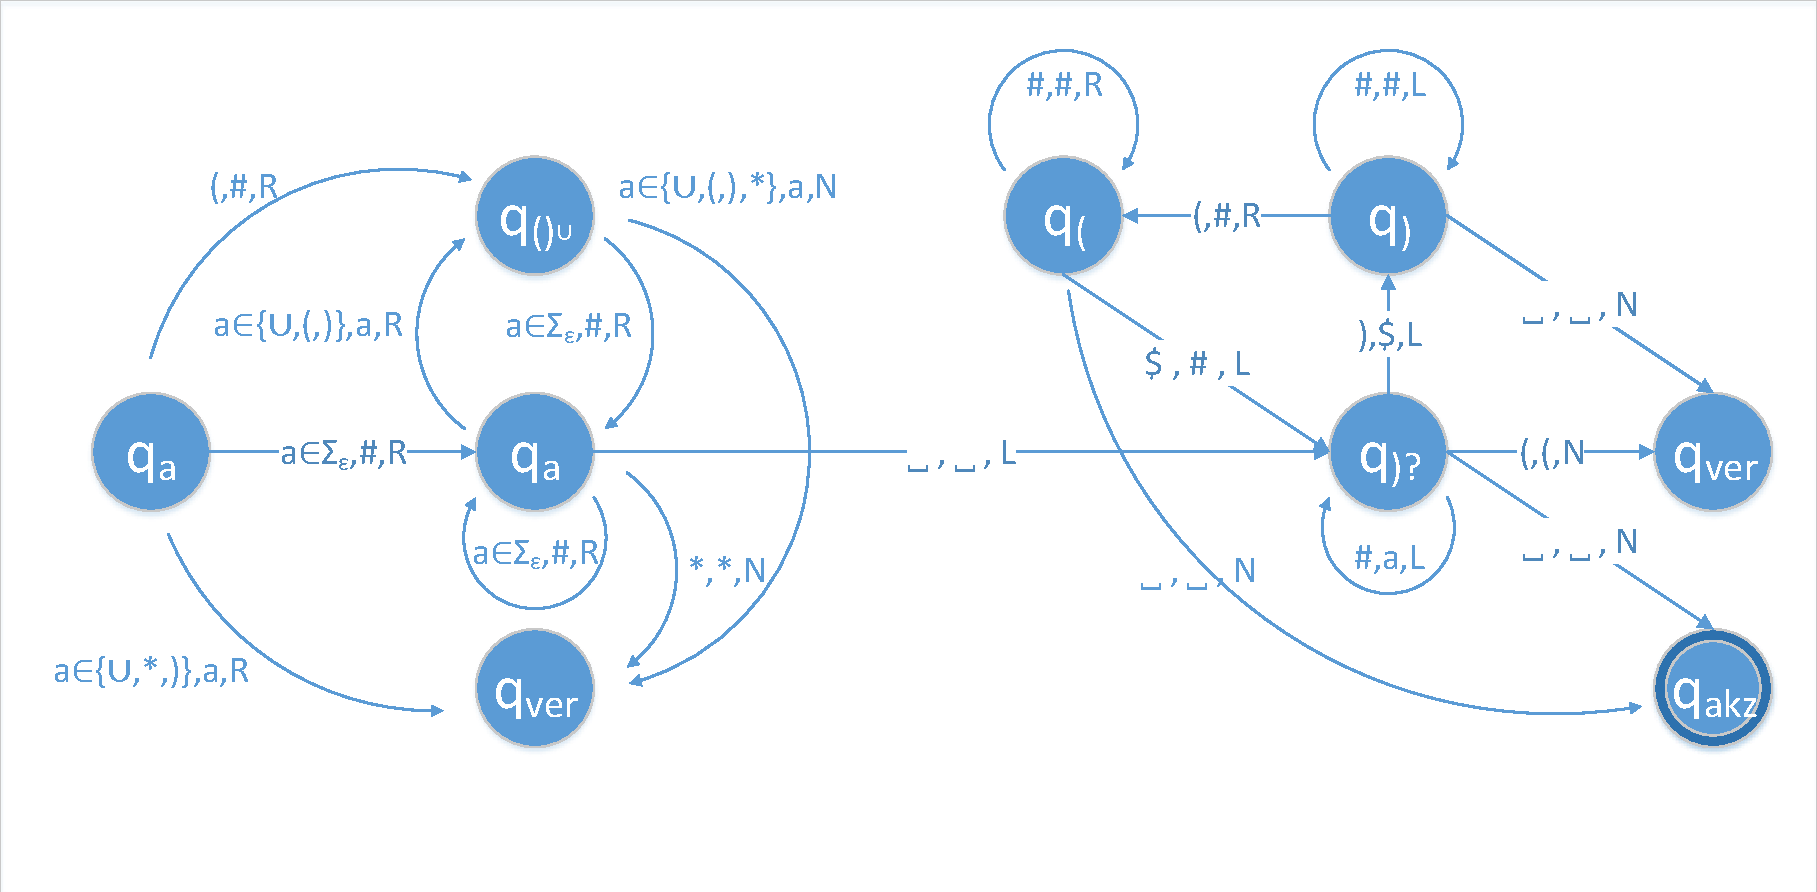
\includegraphics[width=\textwidth,page=1,trim={2 2 2 4},clip]{diagramme.pdf}
\end{minipage}
Das Überschreiben des Bandes mit der Ausgabe haben wir uns hier erspart, aber es ist klar, wie man die TM erweitern kann, sodass die entsprechenden Rückgabewerte auf das Band geschrieben werden.

\section*{Aufgabe 5 - \textit{Reduktionen}}

\begin{enumerate}
	\item Seien $X, R$ formale Sprachen. Ferner sei $R$ reguläre Sprache und es gelte $X \le R$, also $\exists f: \Sigma_X \to \Sigma_R : w\in X \Leftrightarrow f(w) \in R$.
	
	Offenbar ist $X$ dann nicht notwendigerweiße ebenfalls reguläre Sprache. Dazu konstruieren wir folgendes Gegenbeispiel: Sei $X := \{0^n1^n | n \ge 0 \}$ und wähle $f$ mit:
	\begin{equation}
		f(w) := \begin{cases}
		0, &\exists n \ge 0 : w = 0^n1^n \\
		1, &\text{sonst}
		\end{cases}
	\end{equation}
	
	Dabei ist $f$ total und ferner Turing-berechenbar. Als Beweis der Turing-Berechenbarkeit geben wir eine Turing-Maschine an, die dies leistet:
	
	\begin{minipage}{\textwidth}
		\centering\includegraphics[width=0.75\textwidth,page=2,trim={2 2 2 4},clip]{diagramme.pdf}
	\end{minipage}
	
	Weiterhin sei $\Sigma_R := \{0,1\}, R:= \{0\}$. Offenbar gilt $X \le R$:
	\begin{equation}
		\begin{cases}
		w \in X \Rightarrow \exists n \ge 0 : 0^n 1^n = w \Rightarrow f(w) = 0 \in R\\
		w \not\in  X \Rightarrow f(w)=1 \not\in R
		\end{cases}
	\end{equation}
	
	Damit haben wir gerade ein $f$ konstruiert, sodass $w \in X \Leftrightarrow f(w) \in R$, also $X \le R$. Nach Konstruktion ist aber $X$ nicht-regulär und $R$ ist trivialerweise regulär.
	
	\item Sei $A$ semientscheidbar und $A \le A^C$. Dann ist $A$ auch entscheidbar.
	
	Dies zeigen wir wie folgt: Da $A$ semientscheidbar ist, ist die partielle Funktion $\chi^*_A$ Turing-berechenbar. Zur Erinnerung:
	\begin{equation}
		\chi^*_A(w) := \begin{cases}
		1, &w \in A\\
		\text{n. def.}, &\text{sonst}
		\end{cases}
	\end{equation}
	
	Wegen $A \le A^C$ gilt ferner: dass es eine totale, Turing-berechenbare Funktion $f : \Sigma_A^* \to \Sigma_A^*$ gibt sodass $w \in A \Leftrightarrow f(w) \in A^C$. Damit gilt aber:
	
	\begin{equation}
		(\chi_A^* \circ f) (w) = \chi_A^* (f(w)) = \begin{cases}
		1, &f(w)\in A \Leftrightarrow w \in A^C\\
		\text{n. def.}, &\text{sonst}
		\end{cases}
	\end{equation}
	
	Da $f$ total und Turing-berechenbar ist, hält die zugehörige Turing-Maschine $M_f$ immer und da ferner eine TM $M$ existiert, die $\chi_A^*$ berechnet, lässt sich eine TM konstruieren, die bei Eingabe $w$ gemäß Programm von $M_f$ den Wert $f(w)$ berechnet und anschließend hierauf die Berechnung von $\chi_A^*$ gemäß Programm von $M$ durchführt. Somit ist $(\chi_A^* \circ f)$ Turing-berechenbare Funktion. Wir modifizieren die Funktion nun noch dahingehend, dass das Ergebnis der Berechnung, falls definiert, durch die partielle Projektionsfunktion $P_0$ auf 0 proziziert wird, sodass $(P_0 \circ \chi_A^* \circ f)(w) = 0$ für $w \in A^C$. (Das ist ebenfalls eine Turing-berechenbare Funktion, die zu jeder Eingabe 0 die Ausgabe 0 produziert.)\\
	
	Nun können wir eine 2-Band-TM konstruieren, welche auf Band 1 ein Eingabewort $w \in \Sigma^*$ erhält, dieses auf Band 2 kopiert und anschließend parallel auf Band 1 $\chi_A^*(w)$ und auf Band 2 $(P_0 \circ \chi_A^*\circ f)(w)$ berechnet. Da $w\in A \lor w \in A^C$ hält die Berechnung auf einem der Bänder immer an und wir können die Übergangsfkt. derart definieren, dass sobald die Berechnung auf einem Band anhält der Rückgabewert dieses Bandes auf Band 1 geschrieben wird und die Berechnung terminiert. Damit haben wir eine TM beschrieben, welche gerade die charakteristische Funktion $\chi_A$ berechnet:
	\begin{equation}
		\chi_A = \begin{cases}
		\chi_A^*(w) = 1, w \in A\\
		(P_0\circ \chi_A* \circ f) (w) = 0, w\not\in A
		\end{cases}
	\end{equation}
	
	Somit ist $A$ entscheidbar und wir sind fertig.
	
	
\end{enumerate}


\end{document}